\title{Improving Wireless Internet Access in a Campus Environment}
\author{
        Christopher Desnoyers\\
        cjdesno@mit.edu
            \and
        Tristan Honscheid\\
        tristanh@mit.edu
            \and
        Robert Rusch\\
        rusch@mit.edu
}
\date{\today}

\documentclass[11pt,twocolumn]{article}

\usepackage{graphicx}

\begin{document}
\maketitle

\section{Introduction}
\subsection{Problem}
\indent Campus Wi-Fi networks are critical to the operation of a modern university. Such networks may be required to serve tens of thousands of users
through several thousand access points, with high expectations of scalability, reliability, and availability. Despite this, existing 
implementations of 802.11, commonly referred to as Wi-Fi, lack many features that may aid in the smooth operation of such large-scale networks in dynamic 
environments such as a college campus. It is difficult to scale, monitor, and intelligently handle network congestion.
\subsection{802.033}
\indent We seek to propose a new wireless network infrastructure, called 802.033, that implements many features of interest to large network operators.
\subsubsection{Brief System Overview}
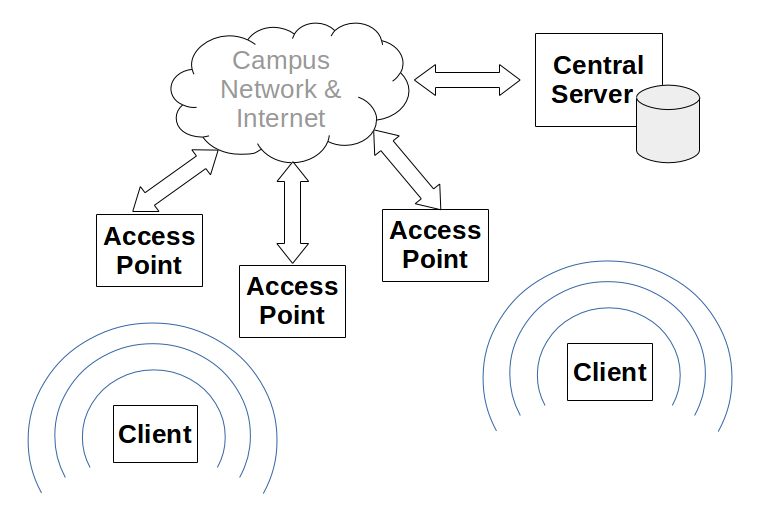
\includegraphics[width=0.5\textwidth]{overview}
\indent The system consists of three main components\\
\begin{enumerate}
	\item \textbf{Central Server:} A central server on the network is used as a hub for the monitoring of network status information. The server also knows
		the locations and network addresses of each Access Point in the system.
	\item \textbf{Access Points:} Access Points are radio-enabled networked devices capable of connecting Clients to the network. They are
		able to execute customized software for handling connections and congestion.
	\item \textbf{Clients:} The Client is the software on the end-user's device that communicates wirelessly to the network and sends connection information and
		user data to Access Points. The Client is able to determine and communicate the user's bandwidth requirement.
\end{enumerate}
\indent Our system provides the following improvements:\\
\subsubsection{Enhanced Monitoring and Diagnostics}
\indent Because campus networks are large both in terms of users and geographic coverage, maintenance, monitoring, and diagnostics can quickly become a
difficult task. Our system seeks to ease such burdens by incorporating an automatic monitoring system that reports detailed statistics to a central
server for archiving. Such statistics include data on Access Point (AP) utilization, user transfers to other AP's, and user (dis)satisfaction reports.\\
\indent Such data allows network operators to diagnose or troubleshoot issues. In the long term, it also allows them to discover and forecast trends that
identify areas of insufficient coverage or high user dissatisfaction. Analysis of this data can guide the installation of future Access Points.
\subsubsection{Congestion Management}
\indent To enhance network utilization and user satisfaction, our wireless network performs congestion management. Access Points track the requested
and actual bandwidth of each Client and can throttle connections or transfer Clients to other, less-congested Access Points as needed. In case no
suitable Access Point is within wireless range, the system can recommend a new Access Point within a brief walking distance (approx. 500 feet).
\subsubsection{Scalability}
\indent Our system is designed to be scalable. This goal has been achieved by concentrating most of the network's intelligence at the Access Point
level. Because the number of Access Points grows with the size of the network, there should be no single point for total failure. \\
\indent As little functionality as possible has been implemented in the Central Server. The Central Server serves only occasional Access Point look-ups (to
find neighboring Access Points, for example) and as a place to store monitoring data. Because there is only one Central Server, this does prevent the 
system from scaling arbitrarily large, but should not be an issue in any reasonably-sized network. 

%System Design
\section{System Design}

%Rusch
\subsection{Client Connections}

\indent
The process for connecting Clients to Access Points is designed to quickly connect the Client to an AP that can provide sufficient bandwidth for 
the client.\\
\indent
When the client first starts or when it needs to reconnect to the wireless network, the Client briefly listens for two types of packets broadcasted 
by each Access Point on its appropriate data channel:
\begin{enumerate}
	\item \textbf{Heartbeat Packets} to determine in-range AP's and the data channel that those AP's are using.
	\item \textbf{Congestion Broadcast Packets} sent out by each AP noting the current congestion at that AP. This packet uses $meta=0xA0$ and is therefore
	not user data.
\end{enumerate}
\indent
The Client, using the information from these packets, then communicates with the least congested AP over its data channel 
\footnote{Signal strength is not considered when choosing a connection as it does not affect the throughput, as stated in the project 
description.}. In the case that all AP's are fully congested, the Client connects to the AP with the greatest signal strength.\\
\indent
Once connected, the Client sends a Connection Request Packet (CRP) to the AP over its data channel that includes (1) a list of all visible AP's by 
MAC address and (2) the Client's requested throughput. \\
\indent
The AP receives the CRP and then determines if it possess sufficient bandwidth for the throughput requested by the Client. If it does, the AP 
establishes a connection and links the Client to the Internet. Otherwise, the AP will query the other visible AP's listed in the CRP over 
the wired network to see if they can support this Client. If another AP has sufficient bandwidth, the originating AP will request 
that the distant AP reserve space for the Client before instructing the Client to connect to the distant AP. Space is explicitly reserved for the 
Client to prevent the race condition where multiple AP's direct Clients to the same Access Point.\\
\indent
If none of the listed Access Points visible to the Client are able to take the Client's connection, the AP, communicating over the wired network, will 
sequentially ask neighboring Access Points within 500 ft if they are able handle the bandwidth requested by the Client. The AP will then direct the client to the closest AP 
capable of handling the requested bandwidth. The building number and room number of that AP will be provided. Because the user will require some transit time when moving into the range 
of the distant AP, the originating AP will request the distant AP to reserve bandwidth. This reservation will time out after several minutes in case the user
chooses not to move. \\

\subsubsection{Adjusting Clients}
\indent
As the load on a particular access point increases sharply, such that the AP may shortly overload, the AP must re-adjust its load. Clients using the highest amounts 
bandwidth are the first to be adjusted, as affecting one large user causes less unhappiness than affecting many smaller users. \\
\indent
When adjustment needs to happen, the AP knows which other AP's each client sees thanks to the list sent in the Connection 
Request Packet. Thus, the AP can contact those AP's and query whether they can support this Client. If so, the 
Client is transferred as done before in the previous section. If none of the AP's within range of the Client 
are able to take the user, the user will have their bandwidth throttled to re-distribute available bandwidth. If the user 
reports unhappiness through the Client after being throttled, the AP will query the AP's in its neighbor list and direct 
the client to the closest suitable AP.
%/Rusch

\subsection{Use Cases}
We considered several use cases during the design of this system.
\subsubsection{Single Client, Empty Network}
\indent This use case represents the most optimal conditions: no congestion and only one Client. In this case, the Client will choose one of many available 
and suitable Access Points within wireless range using the heartbeat and congestion broadcasts. The Access Point will accept the connection directly, and the 
Client gets connected to the Internet.\\
\indent However, should congestion arise in the future, the Access Point already knows which other AP's this Client can see. This makes it easy for the AP to
shed this user to another AP visible to the user.
\subsubsection{Lecture Hall}
\indent In this use case, a large number of students quickly enter a lecture hall. The system must be able to quickly establish many connections. Such a location
will also likely have multiple Access Points. \\
\indent Our system is able to handle this situation thanks to two design features:
\begin{enumerate}
	\item \textbf{Client Chooses Best AP First:} Because the client monitors the frequent Congestion Broadcast Packets, it is able to automatically make its
	initial connection request to the best available AP, reducing the need for the connection to be moved elsewhere.
	\item \textbf{Reservations to Avoid Race Conditions:} As Clients are moved between Access Points, originating AP's reserve bandwidth in the new AP for the
	Client. This avoids the scenario where multiple Clients are transferred to one Access Point without enough available bandwidth for all of them.
\end{enumerate}
\subsubsection{Corridor}
\indent In a corridor, connections will experience high turn-over as users pass Access Points quickly while walking. Having to switch Access Points in this case
is inevitable, as they will all eventually go out-of-range and cost the user one second to change due to the hardware. However, our design features an 
inexpensive software-side connection process. It does not take long for our system to process a connection or find another suitable Access Point.\\
\indent Future revisions may include the ability for Clients to monitor signal strengths, and automatically register with upcoming AP's in advance, and reserver badnwidth there.
\end{document}


